\documentclass{article}
\usepackage{amsmath}

\usepackage{graphicx}

\usepackage{listings}
\usepackage{color}
\definecolor{dkgreen}{rgb}{0,0.6,0}
\definecolor{gray}{rgb}{0.5,0.5,0.5}
\definecolor{mauve}{rgb}{0.58,0,0.82}
\lstset{frame=tb,
  language=R,
  aboveskip=3mm,
  belowskip=3mm,
  showstringspaces=false,
  columns=flexible,
  basicstyle={\small\ttfamily},
  numbers=none,
  numberstyle=\tiny\color{gray},
  keywordstyle=\color{blue},
  commentstyle=\color{dkgreen},
  stringstyle=\color{mauve},
  breaklines=false,
  breakatwhitespace=true,
  tabsize=3
}

\title{SDS385 Fall '16: Statistical Models For Big Data\\Exercises 04 - Putting it all together\\on some biggish data}
\author{Matteo Vestrucci}
\date{October 3rd 2016}
\begin{document}
\maketitle
\bigskip\bigskip\bigskip

\subsubsection*{A)}

Running the code in appendix, we can observe how all the different features we presented for the stochastic gradient descent can speed up the algorithm. The first implementation of AdaGrad in R uses only the sparse matrices trick: it runs on my laptop through all the training dataset in 42 seconds, with a prediction error on the test data of 1.11\%.

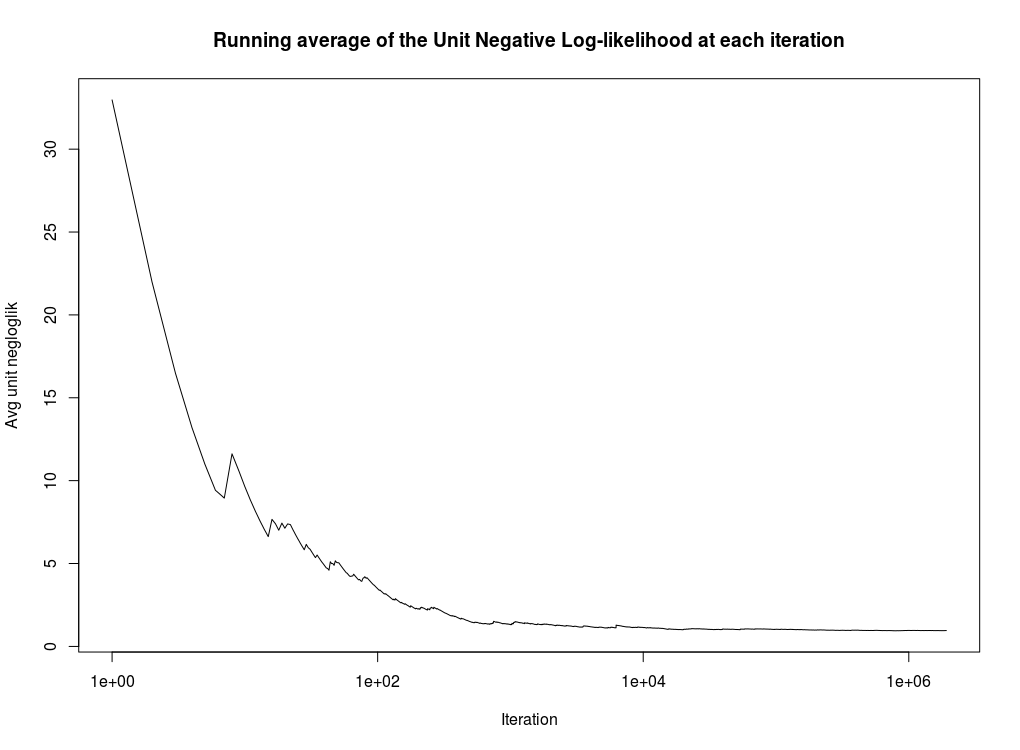
\includegraphics[width=\textwidth]{Rplot_biggish01.png}

In the second implementation I added also the $L^2$ norm penalization for the covariates. It scales on $\lambda$ and to choose it I coded a cross-validation based on a partition of ten pieces of the training set. To cross-validate the values of $\lambda$, the algorithm leaves out one of the ten splits of the training dataset at each iteration to estimate the error. Notice that the values here refer to $1-\lambda$.

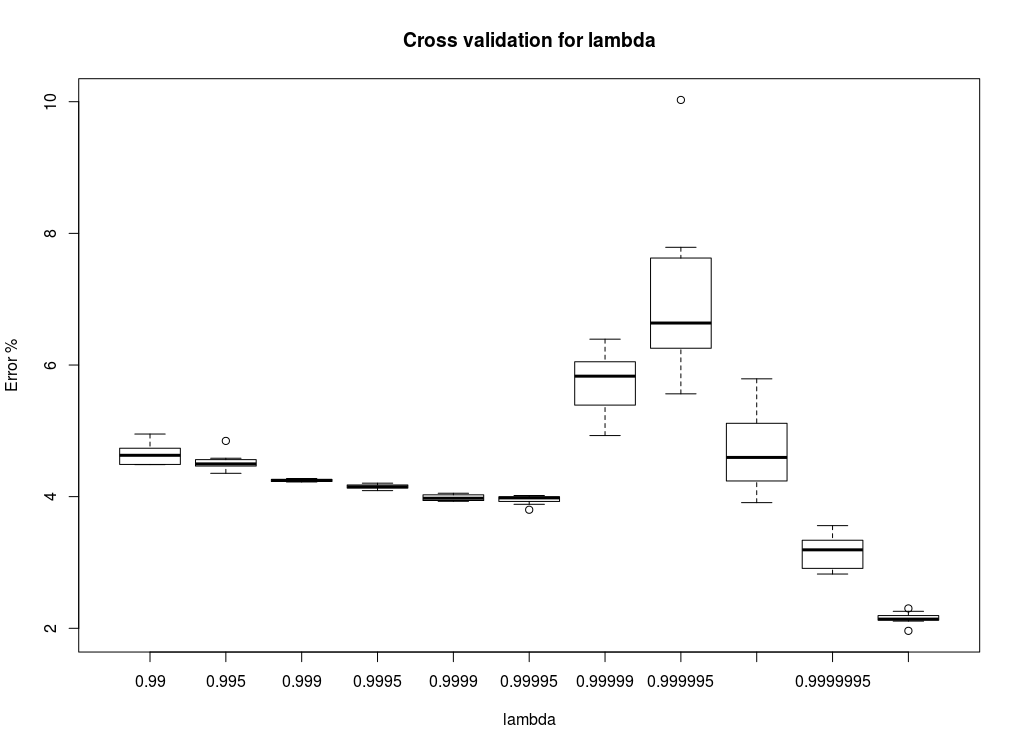
\includegraphics[width=\textwidth]{Rplot_biggish02.png}

\begin{center}
\begin{tabular}{ll}
lambda     &error\\
0.9900000  &4.64\\
0.9950000  &4.52\\
0.9990000  &4.25\\
0.9995000  &4.15\\
0.9999000  &3.99\\
0.9999500  &3.95\\
0.9999900  &5.77\\
0.9999950  &7.04\\
0.9999990  &4.72\\
0.9999995  &3.16\\
0.9999999  &2.15
\end{tabular}
\end{center}

Interestingly the resulting plot suggests that we shouldn't apply any penalization. Finally the third implementation uses $\lambda=0$ and is coded in C++. The error rate is still 1.11\% because the algorithm is deterministic, but it runs considerably faster on my laptop: one full passage on the training dataset takes only 9 seconds.

\newpage

\subsubsection*{CODE)}

%[basicstyle=\tiny]
\begin{lstlisting}
library(Matrix)
library(microbenchmark)
library(Rcpp)
library(RcppArmadillo)
library(compiler)
enableJIT(3)

AdaGrad_biggish<-function(y,X_dim,X_p,X_j,X_x,alpha0,beta0,stepsize,ada_eps){
  n<-X_dim[1]
  p<-X_dim[2]
  unit_negloglik<-numeric(n)
  grad_const<-0
  gradient<-rep(0,p)
  diag_G_const<-ada_eps
  diag_G<-rep(ada_eps,p)
  new_diag_G<-0
  i<-0
  j_start<-0
  j_end<-0
  active_Xs<-0
  values_Xs<-0
  value_y<-0
  values_beta<-0
  Xtbeta<-0
  expbeta<-0
  for(i in 1:n){
    j_start<-X_p[i]+1
    j_end<-X_p[i+1]
    active_Xs<-X_j[j_start:j_end]+1
    values_Xs<-X_x[j_start:j_end]
    value_y<-y[i]
    values_beta<-beta0[active_Xs]
    Xtbeta<-sum(values_Xs*values_beta)+alpha0
    expbeta<-1+exp(-Xtbeta)
    unit_negloglik[i]<-(1-value_y)*Xtbeta+log(expbeta)
    grad_const<-1/expbeta-value_y
    diag_G_const<-diag_G_const+grad_const^2
    alpha0<-alpha0-stepsize/sqrt(diag_G_const)*grad_const
    gradient<-values_Xs*grad_const
    new_diag_G<-diag_G[active_Xs]+gradient^2
    diag_G[active_Xs]<-new_diag_G
    beta0[active_Xs]<-values_beta-stepsize/sqrt(new_diag_G)*gradient}
  return(list(alphahat=alpha0,betahat=beta0,unit_negloglik=unit_negloglik))}

X_dim<-readRDS("url_X_training_dim.rds")
X_p<-readRDS("url_X_training_p.rds")
X_j<-readRDS("url_X_training_j.rds")
X_x<-readRDS("url_X_training_x.rds")
y<-readRDS("url_y_training_vec.rds")

alpha0<-0
beta0<-rep(0,X_dim[2])
stepsize<-0.1
ada_eps<-0.0000001

temp<-date()
res_adagrad_biggish<-AdaGrad_biggish(y,X_dim,X_p,X_j,X_x,alpha0,beta0,stepsize,ada_eps)
temp;date()

res_adagrad_biggish$alphahat
summary(res_adagrad_biggish$betahat)

X_test<-readRDS("url_X_test.rds")
y_test<-readRDS("url_y_test.rds")

alphaXbeta<-res_adagrad_biggish$alphahat+X_test%*%res_adagrad_biggish$betahat
predictions<-(1/(1+exp(-alphaXbeta))>0.5)
error<-round(sum((y_test-predictions)^2)/length(y_test)*100,2)
paste(100-error,"% correct, ",error,"% wrong",sep="")

plot(res_adagrad_biggish$unit_negloglik,
     main = "Unit Negative Log-likelihood at each iteration",
     xlab="Iteration",ylab="Unit negloglik",type="l")

plot(res_adagrad_biggish$unit_negloglik[(X_dim[1]-5000):(X_dim[1])],
     main = "Unit Negative Log-likelihood at each iteration",
     xlab="Iteration",ylab="Unit negloglik",type="l")

update_exp_avg<-function(old,new,w){
  result<-old*w+new*(1-w)
  return(result)}

exp_avg_biggish<-res_adagrad_biggish$unit_negloglik
exp_avg_biggish[exp_avg_biggish==Inf]<-1000
for(i in 2:X_dim[1]){
  exp_avg_biggish[i]<-update_exp_avg(exp_avg_biggish[i-1],exp_avg_biggish[i],0.999)}
plot(exp_avg_biggish,
     main = "Exponential average of the Unit Negative Log-likelihood at each iteration",
     xlab="Iteration",ylab="Avg unit negloglik",type="l")

plot(exp_avg_biggish,
     main = "Exponential average of the Unit Negative Log-likelihood at each iteration",
     xlab="Iteration",ylab="Avg unit negloglik",type="l",log="x")

update_run_avg<-function(old,new,w){
  result<-(old*(w-1)+new)/w
  return(result)}

running_avg_biggish<-res_adagrad_biggish$unit_negloglik
running_avg_biggish[running_avg_biggish==Inf]<-1000
for(i in 2:X_dim[1]){
  running_avg_biggish[i]<-update_run_avg(running_avg_biggish[i-1],running_avg_biggish[i],i)}
plot(running_avg_biggish[-1],
     main = "Running average of the Unit Negative Log-likelihood at each iteration",
     xlab="Iteration",ylab="Avg unit negloglik",type="l",log="x")

AdaGrad_cv<-function(nsplits,lambda,y,X_dim,X_p,X_j,X_x,alpha_init,beta_init,stepsize,ada_eps){
  n<-X_dim[1]
  p<-X_dim[2]
  h<-0
  splits_errors<-numeric(nsplits)
  for(h in 1:nsplits){
    alpha0<-alpha_init
    beta0<-beta_init
    grad_const<-0
    gradient<-rep(0,p)
    diag_G_const<-ada_eps
    diag_G<-rep(ada_eps,p)
    new_diag_G<-0
    i<-0
    j_start<-0
    j_end<-0
    when_active<-rep(0,p)
    delayed_pena<-0
    active_Xs<-0
    values_Xs<-0
    value_y<-0
    values_beta<-0
    Xtbeta<-0
    expbeta<-0
    train<-which((1:n)%%nsplits+1!=h)
    ntrain<-length(train)
    test<-which((1:n)%%nsplits+1==h)
    ntest<-length(test)
    for(i in 1:ntrain){
      j_start<-X_p[train[i]]+1
      j_end<-X_p[train[i]+1]
      active_Xs<-X_j[j_start:j_end]+1
      delayed_pena<-i-1-when_active[active_Xs]
      when_active[active_Xs]<-i
      values_Xs<-X_x[j_start:j_end]
      value_y<-y[train[i]]
      values_beta<-beta0[active_Xs]*lambda^delayed_pena
      Xtbeta<-sum(values_Xs*values_beta)+alpha0
      expbeta<-1+exp(-Xtbeta)
      grad_const<-1/expbeta-value_y
      diag_G_const<-diag_G_const+grad_const^2
      alpha0<-alpha0-stepsize/sqrt(diag_G_const)*grad_const
      gradient<-values_Xs*grad_const
      new_diag_G<-diag_G[active_Xs]+gradient^2
      diag_G[active_Xs]<-new_diag_G
      beta0[active_Xs]<-lambda*values_beta-stepsize/sqrt(new_diag_G)*gradient}
    delayed_pena<-i-when_active
    values_beta<-beta0*lambda^delayed_pena
    predictions<-numeric(ntest)
    alphaXbeta<-0
    for(i in 1:ntest){
      j_start<-X_p[test[i]]+1
      j_end<-X_p[test[i]+1]
      active_Xs<-X_j[j_start:j_end]+1
      values_Xs<-X_x[j_start:j_end]
      alphaXbeta<-alpha0+values_Xs%*%beta0[active_Xs]
      predictions[i]<-(1/(1+exp(-alphaXbeta))>0.5)}
    error<-sum((y[test]-predictions)^2)/ntest*100
    splits_errors[h]<-error}
  return(splits_errors)}

temp<-date()
lambda_cv<-c(0.99,0.995,0.999,0.9995,0.9999,0.99995,0.99999,0.999995,0.999999,0.9999995,0.9999999)
nlambda<-length(lambda_cv)
nsplits<-10
errors<-matrix(NA,nrow=nlambda,ncol=nsplits)
colnames(errors)<-paste("split",1:nsplits)
rownames(errors)<-paste(lambda_cv)
for(i in 1:nlambda){
  errors[i,]<-AdaGrad_cv(nsplits,lambda_cv[i],y,X_dim,X_p,X_j,X_x,alpha0,beta0,stepsize,ada_eps)}
temp;date()

boxplot(t(errors),main="Cross validation for lambda",
        xlab="lambda",ylab="Error %")

sourceCpp(file="cpp_functions.cpp")

temp<-date()
res_adagrad_biggish_cpp<-AdaGrad_biggish_cpp(y,X_dim,X_p,X_j,X_x,alpha0,beta0,stepsize,ada_eps)
temp;date()
\end{lstlisting}

\end{document}